%% AgenticAI4HPC 2026 (SC26) submission.
%% Formatted with the official IEEE conference template (IEEEtran, conference).
\documentclass[conference]{IEEEtran}
\IEEEoverridecommandlockouts
% The preceding line is only needed to identify funding in the first footnote. If that is unneeded, please comment it out.
%Template version as of 6/27/2024
\usepackage{cite}
\usepackage{amsmath,amssymb,amsfonts}
\usepackage{algorithmic}
\usepackage{graphicx}
\usepackage{textcomp}
\usepackage{xcolor}
\usepackage{booktabs}
\usepackage{listings}
\def\BibTeX{{\rm B\kern-.05em{\sc i\kern-.025em b}\kern-.08em
    T\kern-.1667em\lower.7ex\hbox{E}\kern-.125emX}}

\definecolor{codebg}{gray}{0.96}
\definecolor{OliveGreen}{HTML}{1E6F3C}
% Visible placeholder for numbers to be filled in after the live runs (E2-E4).
% Search the source for \xx (or the red "xx" in the PDF) to find every open slot.
\newcommand{\xx}{\textcolor{red}{\textbf{xx}}}
\lstset{
  basicstyle=\ttfamily\footnotesize,
  backgroundcolor=\color{codebg},
  breaklines=true,
  columns=fullflexible,
  frame=none,
  xleftmargin=4pt,
  aboveskip=4pt,belowskip=4pt,
}

% Data-derived numbers emitted by the analysis pipeline (harness/analyze_pareval.py).
% Prefer the real values (results copied to pareval_numbers.tex); fall back to
% TBD placeholders so the draft compiles before the study completes. No result
% number is hand-typed in the body.
\IfFileExists{pareval_numbers.tex}{\newcommand{\Lzerorate}{82.8\%}
\newcommand{\Lzeroci}{[71.1, 90.4]}
\newcommand{\Lonerate}{87.9\%}
\newcommand{\Loneci}{[77.1, 94.0]}
\newcommand{\Ltworate}{87.9\%}
\newcommand{\Ltwoci}{[77.1, 94.0]}
\newcommand{\LtwoGain}{5.2\%}
\newcommand{\LtwoOverLone}{+0.0\%}
\newcommand{\NfailSingleShot}{10}
\newcommand{\EoRescued}{3}
\newcommand{\DvRescued}{3}
\newcommand{\Npairs}{58}
\newcommand{\Ndiffer}{0}
\newcommand{\DvOnlyRescued}{0}
\newcommand{\Ntasks}{16}
\newcommand{\Nmodels}{4}
\newcommand{\Nruns}{174}
\newcommand{\Ntypes}{7}
\newcommand{\RobustGraph}{12/12}
\newcommand{\RobustHist}{24/24}
\newcommand{\RobustReduce}{32/42}
\newcommand{\RobustScan}{0/12}
\newcommand{\RobustSearch}{23/24}
\newcommand{\Nfail}{7}
\newcommand{\NfailRace}{0}
\newcommand{\NfailCompile}{1}
\newcommand{\NfailSemantic}{6}
}{% Placeholder macros so the paper compiles before the study has produced data.
% When harness/analyze_pareval.py runs, it emits results/pareval_numbers.tex with
% real \newcommand values; copy that to paper/pareval_numbers.tex and main.tex
% will prefer it over these defaults. No result number is hand-typed in the body.
\newcommand{\Lzerorate}{\textsc{tbd}}
\newcommand{\Lzeroci}{[\textsc{tbd}]}
\newcommand{\Lonerate}{\textsc{tbd}}
\newcommand{\Loneci}{[\textsc{tbd}]}
\newcommand{\Ltworate}{\textsc{tbd}}
\newcommand{\Ltwoci}{[\textsc{tbd}]}
\newcommand{\LtwoGain}{\textsc{tbd}}
\newcommand{\NfailSingleShot}{\textsc{tbd}}
\newcommand{\EoRescued}{\textsc{tbd}}
\newcommand{\DvRescued}{\textsc{tbd}}
\newcommand{\Npairs}{\textsc{tbd}}
\newcommand{\Ndiffer}{\textsc{tbd}}
\newcommand{\DvOnlyRescued}{\textsc{tbd}}
\newcommand{\LtwoOverLone}{\textsc{tbd}}
\newcommand{\RobustGraph}{\textsc{tbd}}
\newcommand{\RobustHist}{\textsc{tbd}}
\newcommand{\RobustReduce}{\textsc{tbd}}
\newcommand{\RobustScan}{\textsc{tbd}}
\newcommand{\RobustSearch}{\textsc{tbd}}
\newcommand{\Ntasks}{\textsc{tbd}}
\newcommand{\Nmodels}{\textsc{tbd}}
\newcommand{\Nruns}{\textsc{tbd}}
}
\IfFileExists{injected_numbers.tex}{\newcommand{\Ninjected}{3}
\newcommand{\NinjectedCaught}{3}
}{%
  \newcommand{\Ninjected}{\textsc{tbd}}\newcommand{\NinjectedCaught}{\textsc{tbd}}}
\IfFileExists{cross_numbers.tex}{\newcommand{\NopenModels}{3}
\newcommand{\NfrontierRaces}{0}
\newcommand{\NopenRaces}{1}
\newcommand{\NopenRescued}{1}
\newcommand{\NraceTasks}{6}
}{%
  \newcommand{\NopenModels}{\textsc{tbd}}\newcommand{\NfrontierRaces}{\textsc{tbd}}%
  \newcommand{\NopenRaces}{\textsc{tbd}}\newcommand{\NopenRescued}{\textsc{tbd}}%
  \newcommand{\NraceTasks}{\textsc{tbd}}}
\IfFileExists{scaling_numbers.tex}{\newcommand{\Ntimed}{63}
\newcommand{\NpathScale}{1}
\newcommand{\NflatScale}{15}
\newcommand{\PctFlatScale}{24\%}
\newcommand{\NflatCompute}{3}
\newcommand{\NgoodScale}{21}
\newcommand{\MeanSpeedupCritical}{5.8}
\newcommand{\MeanSpeedupReduction}{3.6}
}{%
  \newcommand{\Ntimed}{\textsc{tbd}}\newcommand{\NpathScale}{\textsc{tbd}}%
  \newcommand{\NflatScale}{\textsc{tbd}}\newcommand{\PctFlatScale}{\textsc{tbd}}%
  \newcommand{\NflatCompute}{\textsc{tbd}}\newcommand{\NgoodScale}{\textsc{tbd}}%
  \newcommand{\MeanSpeedupCritical}{\textsc{tbd}}\newcommand{\MeanSpeedupReduction}{\textsc{tbd}}}
\IfFileExists{sanitizer_numbers.tex}{\newcommand{\NsanTimed}{63}
\newcommand{\NsanRaces}{0}
\newcommand{\NsanClean}{63}
}{%
  \newcommand{\NsanTimed}{\textsc{tbd}}\newcommand{\NsanRaces}{\textsc{tbd}}%
  \newcommand{\NsanClean}{\textsc{tbd}}}
\IfFileExists{scan_numbers.tex}{\newcommand{\LtwoNoScan}{94.4\%}
\newcommand{\NscanFail}{4}
\newcommand{\NgenuineFail}{3}
}{%
  \newcommand{\LtwoNoScan}{\textsc{tbd}}\newcommand{\NscanFail}{\textsc{tbd}}%
  \newcommand{\NgenuineFail}{\textsc{tbd}}}
\IfFileExists{reward_numbers.tex}{% Auto-generated by harness/reward_selection.py -- do not hand-edit.
\newcommand{\RewardTwoAxis}{4.23}
\newcommand{\RewardRandom}{3.54}
\newcommand{\RewardWorst}{2.43}
\newcommand{\RewardGainPct}{19}
\newcommand{\RewardWorstGain}{1.7}
\newcommand{\NmultiTask}{12}
\newcommand{\RewardSpreadTask}{histogram bin 0-100}
\newcommand{\RewardSpreadLo}{0.33}
\newcommand{\RewardSpreadHi}{6.82}
}{%
  \newcommand{\RewardTwoAxis}{\textsc{tbd}}\newcommand{\RewardRandom}{\textsc{tbd}}%
  \newcommand{\RewardWorst}{\textsc{tbd}}\newcommand{\RewardGainPct}{\textsc{tbd}}%
  \newcommand{\RewardWorstGain}{\textsc{tbd}}\newcommand{\NmultiTask}{\textsc{tbd}}%
  \newcommand{\RewardSpreadTask}{\textsc{tbd}}\newcommand{\RewardSpreadLo}{\textsc{tbd}}%
  \newcommand{\RewardSpreadHi}{\textsc{tbd}}}

\begin{document}

\title{Correct but Not Parallel: What Agent-Generated\\
OpenMP Code Pays to Be Race-Free}

%% ---------------------------------------------------------------------------
%% Author block. Anonymized for submission; real authors are commented out
%% below and will be restored in the camera-ready version.
%% ---------------------------------------------------------------------------
\author{\IEEEauthorblockN{Anonymous Author(s)}
\IEEEauthorblockA{\textit{Affiliation withheld for review} \\
Location withheld \\
email withheld}}

%% \author{\IEEEauthorblockN{1\textsuperscript{st} Given Name Surname}
%% \IEEEauthorblockA{\textit{dept. name of organization (of Aff.)} \\
%% \textit{name of organization (of Aff.)}\\
%% City, Country \\
%% email address or ORCID}
%% \and
%% \IEEEauthorblockN{2\textsuperscript{nd} Given Name Surname}
%% \IEEEauthorblockA{\textit{dept. name of organization (of Aff.)} \\
%% \textit{name of organization (of Aff.)}\\
%% City, Country \\
%% email address or ORCID}
%% }

\maketitle

%% Abstract -- kept free of heavy mathematics per the IEEE template rule; all
%% headline numbers are emitted by the analysis pipeline as macros (never
%% hand-typed).
\begin{abstract}
Agentic AI increasingly writes the parallel code at the heart of high-performance
computing, and increasingly \emph{accepts its own work} through execution
feedback---the same deterministic verifier signal that verification-guided
reinforcement learning uses as its reward in place of human preference. In this
setting a program is accepted, and a post-training reward is paid, only when a
verifier confirms success, so the design of that verifier is the operational
definition of ``good'' parallel code. We ask what it must check. The natural gate is
configuration-robust correctness---agreement with a trusted serial reference under
\emph{every} thread count and repeated run---which catches the silent races a single
execution hides. We build an agent that writes OpenMP code and can invoke a
distribution-aware differential verifier establishing exactly this property, and
evaluate it on the ParEval benchmark with \Nmodels{} state-of-the-art models. Two
findings show a single-axis correctness gate is the wrong reward. First, it is
\emph{saturated}: single-shot generation is already robustly correct \Lzerorate{} of
the time, a repair loop raises this to \Lonerate{}, and replacing the loop's
single-thread check with the full differential verifier leaves it unchanged at
\Ltworate{}---these models seldom write the silent-race failure mode the verifier
targets, a null an independent happens-before detector (Archer) corroborates on every
accepted program. Second, and decisively, it is \emph{gameable by construction}: a
serial program with no parallelism agrees with the reference at every thread count and
scores a perfect \Ltworate{}-equivalent, so a reward defined on outputs is maximized
by deleting the parallelism HPC exists for. Measuring the second axis directly, the
\Ntimed{} programs the verifier accepted as robust span $7.9\times$ speedup down to
$0.33\times$---one accepted program runs three times \emph{slower} on eight threads
than one, and the correctness gate cannot tell it apart from a program that scales. We
argue that verification-guided post-training for HPC therefore needs a second,
\emph{performance} verification gate---does the accepted program actually scale---so
that the reward is two-axis, correctness \emph{and} realized parallelism; the first
has become cheap, and the second is where accepted code now fails. We release the
harness, the two-axis scorer, prompts, and complete agent transcripts.
\end{abstract}


\begin{IEEEkeywords}
agentic AI, large language models, parallel programming, OpenMP, HPC software
engineering, differential testing, correctness, data races
\end{IEEEkeywords}

\section{Introduction}

Agentic AI---systems that plan, reason, and use tools autonomously---is rapidly
being adopted to write the parallel and distributed code at the heart of
high-performance and scientific computing: refactoring legacy kernels, translating
across programming models, and generating the data-processing stages that connect
simulation, analytics, and machine learning~\cite{agentic_hpc}. As it is, these
systems increasingly \emph{accept their own work}: the agent generates a program, an
execution-based tool returns a verdict, and it ships---or repairs and
re-submits---on the strength of that verdict. That same verdict is the signal at the
center of the reinforcement learning that now post-trains code models, where a
deterministic verifier replaces human preference as the reward~\cite{rlvr,grpo}.
This is the setting of \emph{verification-guided} post-training: generation is treated
as a control problem in which a stage of work terminates, and reward is paid, only
when an execution verifier confirms success---an execution-based termination
condition on a temporally abstracted action, or \emph{option}, in the
sense of~\cite{options}. Whether the verifier is consumed as an agent's acceptance
gate or as such an RL reward, it \emph{is} the operational definition of ``good''
parallel code. The reliability question is therefore a question about the verifier:
\emph{what must an execution-based gate check before we should trust---or optimize
toward---the parallel code an agent produces?}

Two properties make this hard for parallel code. First, the correctness of parallel
and distributed code is a \emph{global} property of its execution. Whether a result
is right can depend on how many partitions or threads the work is divided into,
whether an operation imposes a total order, and how partial results are combined
across workers---none of which is visible in the \emph{local} sequence of tokens a
code model attends to. The difficulty is documented: state-of-the-art models are far
less reliable at parallel code than at its serial equivalent~\cite{pareval}, and
generated parallel routines routinely harbor races and nondeterminism that a casual
run does not reveal. Second, and specific to \emph{agentic} systems: an agent that
checks its own work by \emph{executing it once} observes that the program ran and
produced plausible output, and concludes it is correct. But distribution- and
concurrency-semantics bugs need not fail on any single run. The very signal an agent
naturally uses to verify itself---and that an RL loop would reward---can be blind to
a class of bugs that only a change of configuration reveals, and so is the check a
developer most often performs.

Consider an agent asked to compute a histogram---count how many array elements fall
into each of several bins. The agent writes an OpenMP loop that increments a shared
bin array in parallel, runs it once, sees a plausible histogram, and submits. The
program is wrong: multiple threads update the same bin counter without
synchronization, so counts are lost to a data race. But on a single thread the loop
runs sequentially and the histogram is exactly right, and even on several threads the
lost updates may be few enough to look plausible. Nothing in a single run reliably
reveals this---not to a developer who validated once, and not to an agent whose only
tool is to execute and inspect the output. The bug is invisible to exactly the check
that was performed, and any reward computed from that check would certify it.

We frame the property such a signal should establish as \emph{configuration-robust
correctness}: a generated program is robustly correct only if it agrees with a
trusted serial reference under \emph{every} execution configuration---each thread
count and repeated run---rather than under the single configuration that happens to
be tested. The quantity of interest is the \emph{gap} between
\emph{single-configuration correctness}, what an ordinary run observes, and
configuration-robust correctness: programs in this gap pass the check yet are not
robust. This gap is the silent-failure surface---and, crucially for an agent, it is
\emph{actionable}: the right verification tool can expose it.

But a signal that will be \emph{optimized}---by an agent's repair loop, or by an RL
post-training objective built on verifiable rewards~\cite{rlvr,grpo}---can fail as a
specification in two distinct ways, and both organize this paper. It can be
\emph{saturated}: if capable models already satisfy it, a more sensitive correctness
signal supplies no additional gradient, and the effort spent making verification
finer is wasted. And it can be \emph{gameable}: if its optimum is reachable by a
degenerate solution, whatever optimizes it drifts toward that solution. We find the
natural correctness signal for parallel code exhibits \emph{both} pathologies at the
frontier. The saturation is empirical: existing self-repair loops---Self-Debugging
\cite{selfdebug}, Reflexion~\cite{reflexion}, and, in HPC, self-correcting
parallel-code translation~\cite{lassi}---consume a single-configuration signal that is
\emph{in principle} blind to nondeterministic races, yet for frontier models on
standard tasks a distribution-aware signal that is \emph{not} blind changes nothing,
because those models seldom write the bug. The gameability is structural: robust
correctness is a predicate on outputs, and a serial program with every parallel
construct deleted satisfies it perfectly---so the signal is \emph{maximized} by code
that does not parallelize at all. The remedy follows the same verification-guided
logic that motivated the correctness gate: pair it with a second verification-gated
option---a \emph{performance} gate whose termination condition is not ``does it agree
with the reference'' but ``does it actually scale''---so that the reward an agent or
an RL loop optimizes is two-axis, correct \emph{and} parallel. This paper establishes
the evidence for that gate; building and training it is the natural next step
(Section~\ref{sec:discussion}).

We answer with an open, reproducible study built on \textsc{ParEval}~\cite{pareval},
the standard benchmark for LLM-generated parallel code. A tool-using agent writes
OpenMP code and can invoke a small toolbox: compile and run a draft at one thread
count, or \emph{differentially verify} it across a thread-count sweep with repeated
runs against \textsc{ParEval}'s serial reference. Compilation and execution run on a
multi-core cloud machine. We evaluate the agent with state-of-the-art models and, in
a controlled \emph{tool-ablation}, remove the differential verifier to isolate its
contribution; final correctness is always scored by an independent verifier over the
full thread sweep, so the outcome measure does not depend on which tools the agent
was given. Then, holding correctness fixed, we measure the second axis the signal
ignores---realized speedup---on every accepted program.

\noindent This paper makes five contributions.
\emph{First}, we frame the design of the execution-based acceptance signal for
agent-generated parallel code---equivalently, the verifiable reward an RL loop would
optimize---as the central reliability question, and identify the two ways such a
signal fails as a specification: \emph{saturation} and \emph{gameability}
(Section~\ref{sec:metric}). We formalize \emph{configuration-robust correctness} and
the \emph{single-configuration-to-robust gap} as the correctness axis of that signal,
distinct from single-execution functional correctness.
\emph{Second}, we build a distribution-aware differential verifier and expose it as a
first-class tool inside a tool-using agent that writes and self-repairs parallel
code; we release the harness, tasks, prompts, the two-axis scorer, and complete agent
transcripts in line with the SC26 reproducibility initiative
(Sections~\ref{sec:metric}--\ref{sec:setup}).
\emph{Third}, we evaluate the agent with state-of-the-art models on ParEval's OpenMP
tasks and find the correctness signal \emph{saturated}: single-shot generation is
already robustly correct \Lzerorate{} of the time, a repair loop raises this to
\Lonerate{}, and the full differential verifier leaves it unchanged at \Ltworate{},
with Wilson confidence intervals throughout (Section~\ref{sec:results}).
\emph{Fourth}, our controlled tool-ablation returns a \emph{negative and clarifying}
result: for \Nmodels{} state-of-the-art models on standard OpenMP tasks, the
differential verifier does not improve over single-configuration execution, because
these models seldom emit the silent-race failure mode it targets; their errors are
semantic and already visible at one thread, and it is the agent's \emph{repair loop},
not the verifier's granularity, that drives the improvement over single-shot
generation. A positive control with injected races, an independent happens-before
detector (Archer), and an open-weights panel---on which a smaller model ships a
genuine race the verifier catches and repairs---bound the tool's value: it rises
exactly as capability falls (Sections~\ref{sec:results}--\ref{sec:discussion}).
\emph{Fifth}, and most consequential, we show the correctness signal is
\emph{gameable by construction}---a serial program scores perfectly---and measure the
second, performance axis directly: the programs the verifier accepts span
$0.33\times$ to $7.9\times$ speedup on eight threads, one running \emph{slower} in
parallel than serially. Once frontier models make race-freedom cheap, any acceptance
gate or verifiable reward for HPC code must score \emph{both} axes---correctness
\emph{and} realized parallelism---because ``correct but not parallel'' is where
agent-generated HPC code now fails, and an output-only signal cannot see it. We
therefore argue for a two-axis verification-guided reward, adding a \emph{performance
gate} beside the correctness gate, and show on our own data that selecting programs by
correctness alone leaves large speedups on the table that a two-axis reward recovers
(Section~\ref{sec:scaling}, Section~\ref{sec:discussion}).

\section{Configuration-Robust Correctness}
\label{sec:metric}

We formalize the metrics used throughout the paper. The guiding idea is to
separate correctness that a developer (or an agent) can \emph{observe cheaply}---by
running a program once at low parallelism---from correctness that actually
\emph{holds} once the program executes across the parallel configurations a
production run will use.

\subsection{Setup and Notation}
Let $\mathcal{M}$ denote the set of models under evaluation and $\mathcal{T}$ a
set of parallel-programming tasks. Each task $t\in\mathcal{T}$ is specified by a
natural-language prompt with an explicit function contract and is equipped with a
\emph{trusted serial reference} $R_t$: a sequential implementation that defines
the correct output on any input. A model $m$ produces a program
\begin{equation}\label{eq:gen}
G(m,t) \;=\; \textsc{extract}\big(m(\textsc{prompt}(t))\big),
\end{equation}
where $\textsc{extract}(\cdot)$ recovers the code from the response. The generated
program and the reference are compiled into the same driver, which supplies
randomized inputs and adjudicates the program's output against $R_t$.

A parallel program admits a family of \emph{execution configurations}
$\mathcal{K}$. A configuration fixes a degree of parallelism---here an OpenMP
thread count $\tau\in\{1,2,4,8\}$---and a repetition index that re-runs the same
program to expose nondeterminism. Executing program $G$ under configuration
$k\in\mathcal{K}$ yields either a validated output or the failure symbol $\bot$
(a crash or a compilation failure), and the driver reports a per-configuration
correctness indicator
\begin{equation}\label{eq:corr}
\mathrm{corr}(G,k) \;=\;
\begin{cases}
1 & G\text{ runs under }k\text{ and its output matches }R_t\\
  & \text{on every validation input,}\\
0 & \text{otherwise.}
\end{cases}
\end{equation}
Correctness is checked against the serial reference on multiple randomized
inputs, so a program must be right on all of them, not merely on a fixed example.

\subsection{Single-Configuration vs.\ Robust Correctness}
Let $k_0\in\mathcal{K}$ denote the \emph{developer-default} configuration: a
single thread ($\tau{=}1$), the most forgiving setting and the one a quick local
check most naturally uses. Because a single-threaded run executes the parallel
constructs sequentially, it hides precisely the hazards---races,
non-associative combines, order dependence---that only manifest when the work is
actually divided. We define two correctness notions for a generated program $G$:
\begin{align}
\text{single-configuration:}\quad \mathcal{S}(G) &= \mathrm{corr}\big(G,k_0\big),\label{eq:S}\\
\text{configuration-robust:}\quad \mathcal{R}(G) &= \!\!\prod_{k\in\mathcal{K}}\!\! \mathrm{corr}(G,k).\label{eq:R}
\end{align}
$\mathcal{S}$ is what an ordinary single-run check observes; $\mathcal{R}$
requires agreement with the reference under \emph{every} thread count and every
repetition. We also define \emph{configuration-invariance} $\mathcal{I}(G)=1$ iff
$G$ produces identical outputs for all $k$ (regardless of whether they are
correct)---a program can be invariant yet uniformly wrong.

\subsection{Correctness Is Necessary, Not Sufficient: The Second Axis}
\label{sec:secondaxis}
$\mathcal{R}$ has a deliberate blind spot that is central to this paper: it is a
predicate on \emph{outputs}, so it is \emph{maximized by removing parallelism
altogether}. A program that deletes every \texttt{\#pragma}, or wraps the loop body
in one \texttt{critical}, agrees with the serial reference at every thread
count and is therefore configuration-robustly correct---while running no faster,
or slower, than serial code. A correctness metric for parallel code that a serial
program aces is not, by itself, measuring parallel code. We therefore pair
$\mathcal{R}$ with a \emph{performance} axis. For a program that compiles and
validates, let $T(G,p)$ be its wall-time on $p$ threads; its \emph{self-speedup}
is $\mathcal{P}_p(G)=T(G,1)/T(G,p)$ and its parallel efficiency
$\mathcal{P}_p(G)/p$. An acceptance test for agent-generated parallel code needs
\emph{both} axes: $\mathcal{R}(G){=}1$ (robustly correct) \emph{and}
$\mathcal{P}_p(G)$ meaningfully above $1$ (actually parallel). Section~\ref{sec:results}
shows the second axis, not the first, is where accepted code fails.

\subsection{$\mathcal{R}$ Is an Estimator with Bounded Power}
$\mathcal{R}$ in Eq.~\ref{eq:R} is a finite product over a sampled
$\mathcal{K}$, not a decision over the whole configuration space, so it is an
\emph{estimator} of robustness with quantifiable power. If a program fails a given
configuration nondeterministically with per-run probability $p$, then $N$
independent validations detect it with probability $1-(1-p)^N$; conversely,
observing $0$ failures over $N$ runs bounds the latent failure probability above by
$\approx 3/N$ at 95\% confidence (the rule of three). We use this throughout:
we report our null not as ``zero races'' but as an upper bound on the
silent-failure risk, and we characterize the estimator's power against injected
hazards as a function of input size, thread count, and repetitions
(Section~\ref{sec:results}).

\subsection{The Parallel-Correctness Gap}
Aggregating over a population of generated programs, the \emph{robust-correctness
rate} is $\overline{\mathcal{R}}=\mathbb{E}[\mathcal{R}(G)]$ and the
\emph{single-configuration rate} is $\overline{\mathcal{S}}=\mathbb{E}[\mathcal{S}(G)]$.
Their difference isolates programs that pass the developer-default check yet are
not robustly correct:
\begin{equation}\label{eq:delta}
\Delta \;=\; \Pr\!\big[\mathcal{S}(G){=}1 \ \wedge\ \mathcal{R}(G){=}0\big],
\end{equation}
the \emph{parallel-correctness gap}, with associated conditional
$\Pr[\mathcal{R}{=}0\mid\mathcal{S}{=}1]$, the \emph{silent-failure risk}: of
programs that look correct at low parallelism, the fraction actually wrong at some
higher thread count. This gap is the surface of bugs that neither a developer's
single run nor an agent's single-execution check can see.

\subsection{Verdicts and Hazard Classes}
For reporting we assign each program a mutually exclusive verdict:
\emph{robust} ($\mathcal{R}{=}1$); \emph{flaky}
($\exists k:\mathrm{corr}(G,k){=}1$ but $\mathcal{R}{=}0$, i.e.\ correct at some
thread counts or repetitions and not others---the signature of a data race);
\emph{wrong} (compiles and runs but never matches the reference); and
\emph{crash} (fails to compile or run under every configuration). Orthogonally,
we tag each program by the \emph{parallel hazard} it may exhibit, summarized in
Table~\ref{tab:hazards}. Each hazard has a characteristic differential
signature---whether the failure varies across thread counts or is invariant---that
the harness detects automatically.

\begin{table}[t]
\caption{Parallel hazard classes probed by the benchmark and their signature
under differential (thread-swept, repeated) execution. Inv.\ = the wrong result
is invariant across thread counts; \emph{varies} = the result changes with the
thread count or across repetitions.}
\label{tab:hazards}
\centering\footnotesize
\begin{tabular}{@{}p{2.5cm}p{3.1cm}l@{}}
\toprule
Class & Typical cause & signature \\
\midrule
H1 data race        & shared accumulator written without \texttt{reduction}/\texttt{atomic}  & \emph{varies} \\
H2 non-associative combine & reduction whose operator is not associative/commutative as written & \emph{varies} \\
H3 order-dependent selection & ``first''/representative element chosen without a total order & \emph{varies} \\
H4 sequential dependence & scan/recurrence parallelized despite a loop-carried dependence & invariant/varies \\
\bottomrule
\end{tabular}
\end{table}

\subsection{An Agent and Its Verification Tool}
\label{sec:agent}
The metrics above measure single-shot generation. To ask whether an \emph{agent}
can repair its own parallel code, we wrap generation in a standard
propose--observe--repair loop and vary only the \emph{tool} that produces the
observation. Given a task, the agent emits a program; a tool returns an
observation; the observation is appended to the context; the agent revises. The
loop stops when the tool reports success or a repair budget $B$ is exhausted. We
define three tool levels that isolate the value of distribution-aware
verification:
\begin{itemize}
\item \textbf{L0 (single-shot).} No tool; the first program is accepted. This is
the baseline, $\mathcal{S}$/$\mathcal{R}$ of Section~\ref{sec:metric}.
\item \textbf{L1 (execute-once).} The program is compiled and run under the
developer-default configuration $k_0$ ($\tau{=}1$); a crash or compile trace is
returned, but the program is validated at only one thread count, so any program
that runs and matches at $\tau{=}1$ is accepted. This is what an ordinary
execute-and-fix agent observes.
\item \textbf{L2 (differential verify).} The verifier of
Section~\ref{sec:metric} compiles the program and executes it across the thread
sweep with repetitions, checking each run against the serial reference $R_t$ and
returning \textsc{pass} or a specific diagnostic (a failing thread count, a
race-indicating variation across repetitions, or a crash).
\end{itemize}
Only the observation differs across levels; the model, prompt, and budget are
held fixed, so any difference in final correctness is attributable to the
\emph{tool}. We report the robust-correctness rate $\overline{\mathcal{R}}$ of
each level's \emph{final} program and the average number of repair rounds it
consumes.

\section{Benchmark and Experimental Setup}
\label{sec:setup}

\subsection{Tasks}
We build directly on \textsc{ParEval}~\cite{pareval}, the standard benchmark for
LLM-generated parallel code, reusing its function-completion prompts, its
randomized-input drivers, and---crucially---its \emph{serial reference}
implementations as our trusted oracle $R_t$. We draw the OpenMP tasks whose
correct result is sensitive to how the work is parallelized: histograms
(shared-bin updates), reductions (associativity and commutativity of the
combine), scans (loop-carried dependence), and searches (order-dependent
selection). These instantiate the hazard classes of Table~\ref{tab:hazards}. Each
prompt states the required computation and signature but never dictates the
parallelization strategy, so the model must choose a race-free, order-correct
implementation on its own.

\subsection{Oracle and Data}
Correctness is adjudicated by \textsc{ParEval}'s own driver: for each generated
completion the driver compiles the model's function together with the serial
reference, generates randomized inputs, runs both, and reports whether their
outputs agree. Using the benchmark's serial reference as the oracle means the
ground truth is independent of the parallel implementation under test, and the
randomized multi-input validation prevents a program from passing on a single
lucky example. Because the oracle is a sequential program, it is itself immune to
the parallel hazards we study.

\subsection{Differential Verifier and Configurations}
The novel component of our harness is a \emph{distribution-aware differential
verifier}. Rather than validating a completion once, it compiles the program with
OpenMP and executes it across a thread-count sweep $\tau\in\{1,2,4,8\}$ with
repeated runs at each setting, checking every run against the serial reference. A
program is robustly correct only if it validates at every thread count and every
repetition (Eq.~\ref{eq:R}); a result that changes with the thread count, or that
varies across repetitions at a fixed thread count, is the signature of a data
race or an order-dependent computation and is reported as \emph{not robust} with a
diagnostic. Repeated execution is what lets the verifier catch nondeterministic
races that a single validation---\textsc{ParEval}'s default, and an ordinary
agent's execute-and-fix signal---can miss. Compilation and execution run on a
dedicated multi-core cloud VM; the verifier, prompts, and per-run transcripts are
released for reproduction in line with the SC26 reproducibility initiative.

\subsection{Model Panel}
We evaluate \Nmodels{} state-of-the-art instruction-tuned models from a single
provider, spanning a current frontier general-purpose model, its preceding
generation, a code-specialized model, and a higher-reasoning ``pro'' variant---all
accessed through Azure AI Foundry under Entra ID authentication, with no API keys
stored. Holding the benchmark, harness, and prompts fixed, this within-provider
panel spans capability and specialization tiers while controlling for
provider-specific idiom: a tool effect---or its absence---that holds across all
\Nmodels{}, including a model tuned specifically for code, is unlikely to be an
artifact of a single weak or idiosyncratic model. Our harness is model-agnostic and
reaches any deployment through one uniform API. We exploit this to add an
\emph{open-weights} panel---\NopenModels{} models served through an
OpenAI-compatible gateway on a research cluster, spanning a 120B general model and a
27B model---which we run on the race-prone task subset to probe the
capability-dependence of the verifier's value (Section~\ref{sec:crosscap}); a
broader cross-vendor sweep remains future work (Section~\ref{sec:discussion}).
Generation in the baseline condition
is single-shot with no tool use: the model receives the prompt and returns a
completion, which the harness compiles and verifies as-is. Every
generation---system prompt, user prompt, raw response, extracted code, and
verifier feedback---is logged as a reusable artifact.

\subsection{Agentic Tool-Ablation Setup}
For the tool-ablation (Section~\ref{sec:agent}) we run the same
propose--observe--repair agent at levels L0 (single-shot), L1 (execute-once), and
L2 (differential verify), holding the model, prompt, and repair budget $B$ fixed
and varying only the verification tool (Fig.~\ref{fig:pipeline}). The agent completes the task, the tool
returns an observation, and---for L1 and L2---the agent repairs on failure until
the tool reports success or the budget is exhausted. Regardless of condition, the
\emph{final} program of every run is scored by the full differential verifier over
the complete thread sweep, an outcome measure independent of which tool the agent
was permitted to use. Every repair round---the verifier feedback and the revised
program---is logged, so the agent's tool-use and repair trajectory is fully
auditable.

\begin{figure}[t]
\centering
\IfFileExists{../results/figures/fig_pipeline.pdf}
  {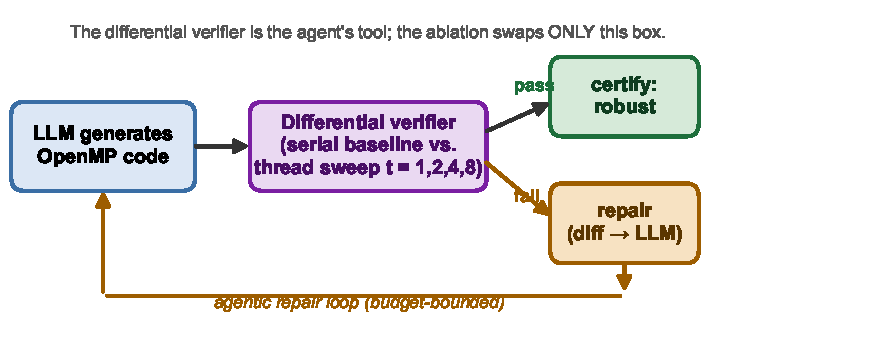
\includegraphics[width=0.99\linewidth]{../results/figures/fig_pipeline.pdf}}
  {\fbox{\parbox{0.8\linewidth}{\centering\vspace{2em}\textsc{[pipeline schematic]}\vspace{2em}}}}
\caption{The agentic pipeline. The model proposes a completion; the tool returns an
observation (nothing at L0, a single-thread pass/fail at L1, or the full
thread-sweep verdict at L2); on failure the agent repairs until the tool reports
success or the budget is spent. Every run's \emph{final} program is scored by the
full differential verifier, independent of the tool the agent could use.}
\label{fig:pipeline}
\end{figure}

\section{Evaluation}
\label{sec:results}

We evaluate over \Nruns{} agentic runs---\Ntasks{} \textsc{ParEval} OpenMP tasks
spanning \Ntypes{} problem families, \Nmodels{} models, and three tool levels---and
report configuration-robust correctness (Eq.~\ref{eq:R}) with Wilson 95\%
confidence intervals throughout. The evaluation is built around a single question:
does a verifier that \emph{observes} many thread counts make an agent's parallel
code more robust than one that observes a single configuration? Our answer is a
precise, instrumented \emph{null}---the differential verifier changed no
outcome---paired with a positive control that proves the instrument is not inert.
We report the null prominently because we designed the study to detect its
opposite, and it did not appear.

\subsection{The Measurement Is a Thread Sweep, Not a Single Run}
Figure~\ref{fig:sweep} contains the study in one plot. For every generated program
we record the validation pass-rate at each thread count $\tau\in\{1,2,4,8\}$
against the serial oracle. Robust model code (green) is \emph{flat}: a program that
is correct at one thread stays correct at eight. The red curve is the failure this
paper is about, and it is not hypothetical---it is a program an open-weights model
actually shipped (Section~\ref{sec:crosscap}): a shared-bin histogram, correct at
one thread and collapsing above it. The title of this paper is the gap between
those two curves. A single-configuration check---\textsc{ParEval}'s default and an
ordinary agent's execute-and-fix signal---samples only the leftmost point, where
the two curves coincide; the differential verifier samples the whole line. For the
frontier models the two curves stayed together, because those models did not write
programs that live in the gap; the red curve shows what happens when a model
does.

\begin{figure}[t]
\centering
\IfFileExists{../results/figures/fig_thread_sweep.pdf}
  {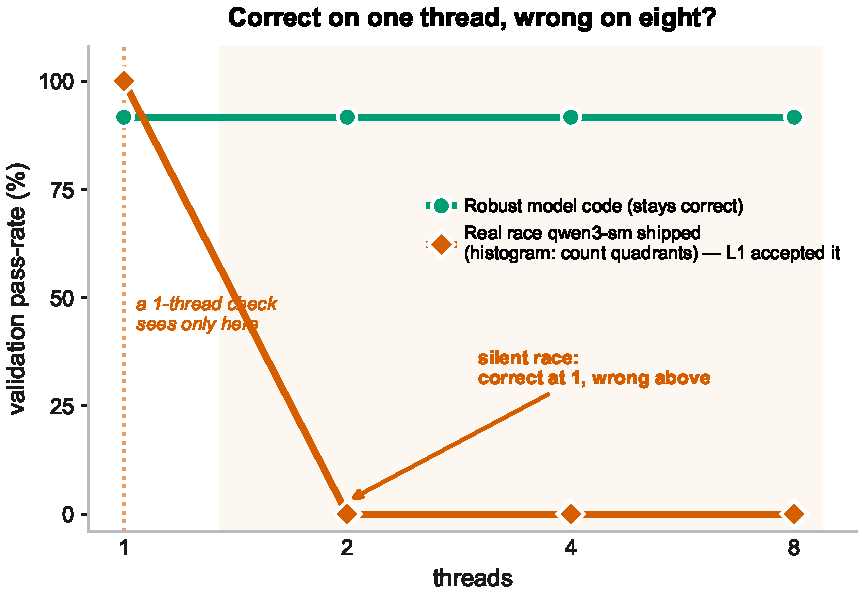
\includegraphics[width=0.92\linewidth]{../results/figures/fig_thread_sweep.pdf}}
  {\fbox{\parbox{0.8\linewidth}{\centering\vspace{2em}\textsc{[thread-sweep figure]}\vspace{2em}}}}
\caption{The study in one plot. Validation pass-rate versus thread count. Robust
model code (green) stays correct at every thread count; the red curve is a
\emph{real} silent race an open-weights model shipped---a shared-bin histogram
that is correct on one thread and wrong on two, four, and eight
(Section~\ref{sec:crosscap}), which the execute-once tool accepted. A one-thread
check sees only $\tau{=}1$ (shaded region is invisible to it).}
\label{fig:sweep}
\end{figure}

\subsection{The Parallel-Correctness Gap---Where It Was Not}
The decisive quantity for a differential verifier is how many generated programs
are of the \emph{silent-race} kind: correct at $\tau{=}1$ yet wrong at some higher
thread count. Across all \Ntasks{}$\times$\Nmodels{} task--model cells we observed
\NfailRace{} such programs. When the models were wrong they were wrong already on a
single thread---never only at higher thread counts: of \Nfail{} failing programs
under the strongest tool level, \NfailSemantic{} disagreed with the reference
already at $\tau{=}1$ and \NfailCompile{} failed to compile; \NfailRace{} were
races. As Section~\ref{sec:hetero} details, most of the $\tau{=}1$ disagreements are
a specification-ambiguity artifact on the scan family (correct parallel code, indexed
against an ambiguous prompt); the genuine residue is a single reduce task.
Where a data race was the natural pitfall---shared
histogram bins, a graph accumulator---the models pre-empted it with the correct
OpenMP idiom (a \texttt{reduction} or an \texttt{atomic}), and those tasks were
robust at every thread count. The gap we set out to measure was, for these models
on these tasks, empty.

\subsection{Tool Ablation: The Repair Loop Helps; The Verifier's Granularity Does Not}
\label{sec:ablation}
Figure~\ref{fig:ablation} and Table~\ref{tab:ablation} report the ablation
(Section~\ref{sec:agent}): the same agent at three tool levels differing only in
the observation the tool returns. Single-shot generation (L0) is robustly correct
\Lzerorate{} of the time (95\% CI \Lzeroci{}). Adding a repair loop driven by an
\emph{execute-once} tool (L1) raises this to \Lonerate{} (95\% CI \Loneci{}).
Replacing that tool with the \emph{differential verifier} (L2) yields \Ltworate{}
(95\% CI \Ltwoci{})---\emph{identical} to L1
($\Delta_{\text{L2--L1}}=\LtwoOverLone{}$). The paired view is sharper than the
aggregate: of the \Npairs{} task--model cells, the number in which execute-once and
differential verification reached a \emph{different} final verdict was \Ndiffer{},
and the number that only the differential verifier rescued was \DvOnlyRescued{}.
The multi-thread signal never changed an outcome. The improvement over single-shot
is therefore attributable to the \emph{repair loop} that L1 and L2 share, not to
the granularity of the verifier: of the \NfailSingleShot{} cells not robust at L0,
execute-once repaired \EoRescued{} and the differential verifier repaired the same
\DvRescued{}. An agent can only fix what its tool lets it
see---but here both tools saw the same failures, because those failures were
visible at one thread.

\begin{figure}[t]
\centering
\IfFileExists{../results/figures/fig_ablation.pdf}
  {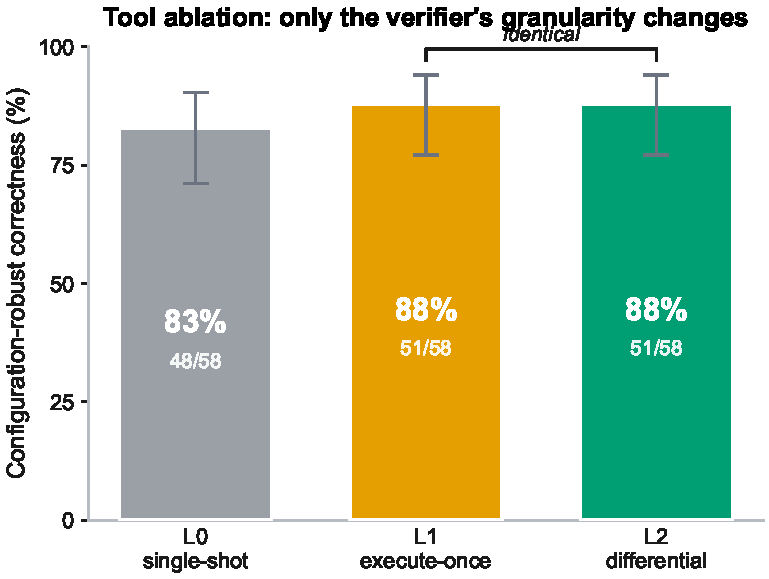
\includegraphics[width=0.82\linewidth]{../results/figures/fig_ablation.pdf}}
  {\fbox{\parbox{0.8\linewidth}{\centering\vspace{2em}\textsc{[ablation figure]}\vspace{2em}}}}
\caption{Tool ablation. Configuration-robust correctness (correct at every thread
count and repeat) with Wilson 95\% CIs; only the verification tool differs across
levels. The repair loop lifts L1 and L2 above single-shot L0, but differential
verification (L2) is indistinguishable from execute-once (L1).}
\label{fig:ablation}
\end{figure}

\begin{table}[t]
\caption{Agentic tool-ablation. Robust correctness with Wilson 95\% CIs; L1 and L2
coincide exactly.}
\label{tab:ablation}
\centering\footnotesize
\begin{tabular}{@{}lcc@{}}
\toprule
Tool level & robust correct. & 95\% CI \\
\midrule
L0 single-shot          & \Lzerorate{} & \Lzeroci{} \\
L1 execute-once         & \Lonerate{}  & \Loneci{}  \\
L2 differential verify  & \Ltworate{}  & \Ltwoci{}  \\
\bottomrule
\end{tabular}
\end{table}

\subsection{Heterogeneity Across Models and Problem Families}
\label{sec:hetero}
The equality of L1 and L2 is not an averaging artifact.
It holds for every model, including the
code-specialized one: no model produced a single case in which the thread sweep and
the single-thread check disagreed, even though the newer models failed \emph{more}
often overall---their losses were semantic and compile errors, not races.
The residual failures were concentrated and, in one family, spurious. Under
differential verification the \NfailSemantic{}+\NfailCompile{} non-race failures
break down as \NscanFail{} on the scan family and only \NgenuineFail{} elsewhere
(all one reduce task, a product-of-inverses combine). We inspected the scan
failures by hand: every model computed the reverse-indexed \emph{suffix} sum
$\text{out}[i]=\sum_{j\ge i}x_j$---a defensible reading of ``reverse prefix
sum''---which is the exact element-wise reverse of \textsc{ParEval}'s reference
(itself an inclusive scan of the reversed input). The models parallelized correctly;
they resolved an ambiguous specification against the reference's example. Excluding
this benchmark artifact, differential-verify robust correctness rises from
\Ltworate{} to \LtwoNoScan{}, and the only genuine failures are three instances of a
single reduce task---so the barrier to correct parallel code here was getting the
sequential algorithm right, not parallelizing it safely.

\subsection{Positive Control: What the Verifier Catches When the Bug Is There}
\label{sec:control}
That the differential verifier changed no outcome invites the obvious question:
does it work at all? To confirm the instrument is not inert we hand-wrote the
\emph{racy} completion a naive or weaker generator would produce for \Ninjected{}
tasks---one per hazard class: an unsynchronized shared-bin histogram, a reduction
accumulated without a \texttt{reduction} clause, and a first-match search with a
racy check-then-write on a shared index. Each is correct on one thread. We verified
each twice with the study's own tool. The execute-once check certified all
\Ninjected{} as robustly correct; the differential verifier rejected all
\NinjectedCaught{}, each failing every sweep run above one thread while passing at
one thread (Table~\ref{tab:injected}). The verifier catches exactly the failure mode a
single-thread check is blind to. The null above is therefore a statement about what
the models \emph{wrote}, not about what the verifier can \emph{see}.

\vspace{2pt}
\noindent\textbf{An independent race detector agrees.} A skeptic might still ask
whether output-differential testing at $\tau\!\le\!8$ simply lacks the power to
expose races that are present. We therefore cross-checked every one of the
\NsanTimed{} accepted programs with a happens-before detector---LLVM
Archer~\cite{archer,sword}, ThreadSanitizer instrumented with the OpenMP runtime's
OMPT annotations---which reasons about the actual synchronization, not just the
output. Archer flagged \NsanRaces{} data races in the model-written code of the
\NsanTimed{} programs the differential verifier certified robust, while correctly
reporting the race in the injected controls and in the open-model histogram of
Section~\ref{sec:crosscap} (27 stack frames in the generated code). Two independent
instruments---one output-differential, one happens-before---agree that these
accepted programs are race-free, which makes the null a statement about the code and
not an artifact of a weak detector.

\begin{table}[t]
\caption{Positive control: injected races, one per hazard class. Each is correct on
one thread; execute-once certifies all, the differential verifier rejects all.}
\label{tab:injected}
\centering\footnotesize
\begin{tabular}{@{}lcc@{}}
\toprule
Injected hazard & execute-once & differential \\
\midrule
Histogram, unsynchronized bins           & \textsc{accept} & \textsc{reject} \\
Reduction, no \texttt{reduction} clause  & \textsc{accept} & \textsc{reject} \\
First-match, racy shared index           & \textsc{accept} & \textsc{reject} \\
\bottomrule
\end{tabular}
\end{table}

\subsection{Beyond the Frontier: A Real Race the Verifier Catches}
\label{sec:crosscap}
The null above is a statement about \emph{capable} models. If differential
verification earns its place by catching silent races, the sharpest test is a
generator that actually writes them. We therefore replayed the \NraceTasks{}
most race-prone tasks through an \emph{open-weights} panel served on a
research cluster (\NopenModels{} models ranging from a 120B general model down to a
27B model), holding the harness, prompts, and differential scorer fixed, and
scored every final program over the full thread sweep
(Fig.~\ref{fig:crosscap}). The capability gradient is exactly the one the null
predicts. The larger open models behaved like the frontier: no silent races,
$L1\!=\!L2$. The smallest model did \emph{not}. On the shared-bin quadrant
histogram it emitted the canonical hazard---a \texttt{local\_bins} accumulator
declared \emph{outside} the parallel region and incremented by every thread, so
the counts are correct on one thread and lost to a data race above it. The
execute-once tool ran it once, saw a plausible histogram, and \textbf{certified
it robust}; the differential verifier ran the sweep, saw it pass at one thread
and fail at two, four, and eight, returned that diagnostic, and the agent
repaired it to a per-thread private accumulator that is robust throughout. Same
model, same task, same repair budget: the only difference was whether the tool
looked at more than one thread count. This is the first \emph{model-emitted}
instance---not an injected control---of the exact failure this paper is about.
Across the open panel the differential verifier caught \NopenRescued{} such
verified silent race(s) that the single-thread check certified, versus
\NfrontierRaces{} on the frontier panel (Fig.~\ref{fig:crosscap}b); we attribute
only genuine pass$@1$/fail$@N$ cases to the verifier and treat the remaining small
$L1$--$L2$ differences on this six-task subset as repair-sampling noise, not race
catches. The mechanism is what matters: the tool's value reappears precisely as
model capability falls.

\begin{figure*}[t]
\centering
\IfFileExists{../results/figures/fig_cross_capability.pdf}
  {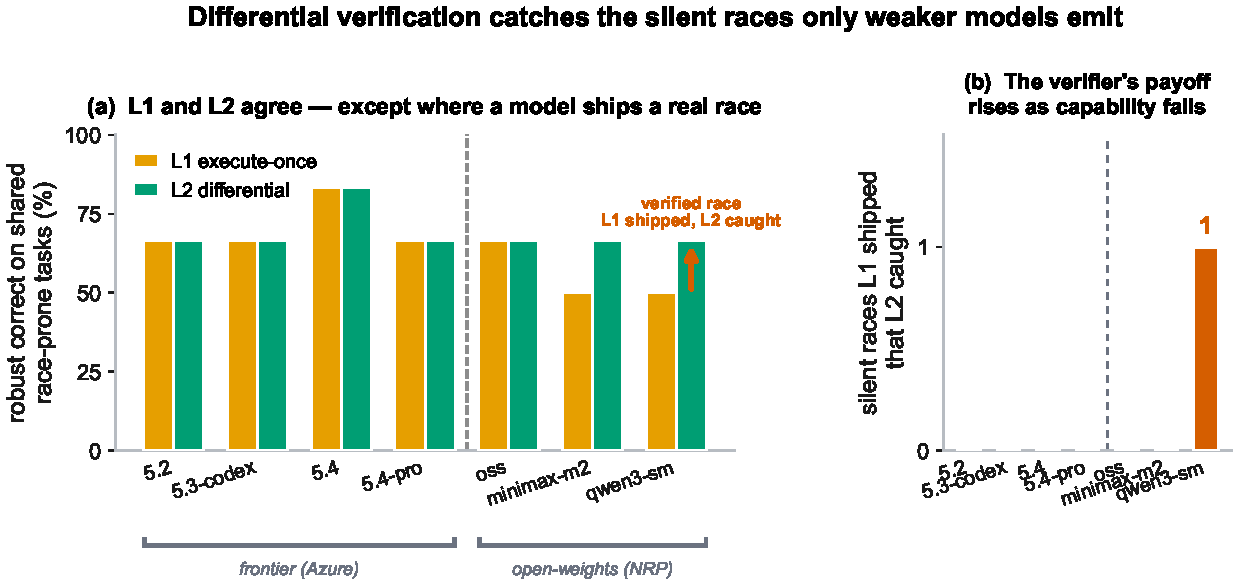
\includegraphics[width=0.94\linewidth]{../results/figures/fig_cross_capability.pdf}}
  {\fbox{\parbox{0.8\linewidth}{\centering\vspace{2em}\textsc{[cross-capability figure]}\vspace{2em}}}}
\caption{The verifier's value is capability-dependent. (a)~Robust correctness on
the shared race-prone tasks, execute-once (L1) vs.\ differential (L2), per model.
Frontier and larger open models show no meaningful gap; the arrow marks the one
\emph{verified} silent race---a shared-bin histogram the smallest open model
shipped, which L1 certified and L2 caught and repaired. (b)~Verified silent races
the single-thread check accepted that the differential verifier rejected: zero for
capable models, rising as capability falls. (Small residual L1--L2 differences in
(a) with no bar in (b), e.g.\ minimax-m2, are repair-sampling noise on this
six-task subset, not race catches.)}
\label{fig:crosscap}
\end{figure*}

\begin{table}[t]
\caption{Open-weights panel on the \NraceTasks{} race-prone tasks. Robust
correctness under L1 (execute-once) and L2 (differential); silent races each model
shipped (correct at one thread, wrong above) that L1 certified; and how many L2
caught. Only the smallest model emits a genuine race---and L2 catches it.}
\label{tab:open}
\centering\footnotesize
\begin{tabular}{@{}lcccc@{}}
\toprule
Open model & L1 & L2 & races shipped & caught by L2 \\
\midrule
gpt-oss-120B & 67\% & 67\% & 0 & 0 \\
MiniMax-M2 & 50\% & 67\% & 0 & 0 \\
Qwen3-27B & 50\% & 67\% & 1 & 1 \\
\bottomrule
\end{tabular}
\end{table}

\begin{figure}[t]
\lstset{basicstyle=\ttfamily\scriptsize,backgroundcolor=\color{codebg},
        breaklines=true,columns=fullflexible,frame=none,aboveskip=2pt,belowskip=1pt,
        escapeinside={(*@}{@*)}}
\textbf{\footnotesize L1 execute-once \textemdash{} shipped; the 1-thread check passed}
\begin{lstlisting}
void countQuadrants(vector<Point> const& pts,
                    array<size_t,4>& bins){
  bins = {0,0,0,0};
  array<size_t,4> local_bins;        // (*@\textcolor{red}{\bfseries shared: declared OUTSIDE omp parallel}@*)
  #pragma omp parallel
  { local_bins = {0,0,0,0};
    #pragma omp for nowait
    for (size_t i=0;i<pts.size();++i) local_bins[q(pts[i])]++; // (*@\textcolor{red}{race}@*)
    #pragma omp critical
    for(int k=0;k<4;k++) bins[k]+=local_bins[k]; }}
\end{lstlisting}
\vspace{-1pt}
{\scriptsize\ttfamily verifier: t1=2/2\; \textcolor{red}{t2=0/2\; t4=0/2\; t8=0/2}\;\(\Rightarrow\)\;\textcolor{red}{NOT\_ROBUST}}

\vspace{4pt}
\textbf{\footnotesize L2 differential \textemdash{} the sweep failed; the agent repaired it}
\begin{lstlisting}
  #pragma omp parallel
  { array<size_t,4> local_bins={0,0,0,0}; // (*@\textcolor{OliveGreen}{\bfseries private: declared INSIDE omp parallel}@*)
    #pragma omp for nowait
    for (size_t i=0;i<pts.size();++i) local_bins[q(pts[i])]++;
    #pragma omp critical
    for(int k=0;k<4;k++) bins[k]+=local_bins[k]; }
\end{lstlisting}
\vspace{-1pt}
{\scriptsize\ttfamily verifier: \textcolor{OliveGreen}{t1=2/2\; t2=2/2\; t4=2/2\; t8=2/2}\;\(\Rightarrow\)\;\textcolor{OliveGreen}{ROBUST}}
\caption{The verified race, from the logs (Qwen3-27B on \texttt{count\_quadrants};
transcripts released). \textbf{Top:} the execute-once agent declares the
accumulator \emph{outside} \texttt{omp parallel}---so all threads share it---but
its one-thread check passes, and it ships. \textbf{Bottom:} given the differential
tool, the same agent sees the thread sweep fail above one thread and moves the
declaration \emph{inside} the region (per-thread private), which is robust. Sweep
lines are the tool's real logged output.}
\label{fig:casestudy}
\end{figure}

\subsection{Correct but Not Parallel: The Second Axis Is Where Accepted Code Fails}
\label{sec:scaling}
The differential verifier settles the correctness axis; it is silent on the second
axis of Section~\ref{sec:secondaxis}. We measured it directly: for every one of the
\Ntimed{} programs the verifier accepted as robust, we compiled the model's code
against \textsc{ParEval}'s timing driver at a size large enough to amortize thread
overhead and recorded self-speedup $\mathcal{P}_p$ across the same sweep
$p\in\{1,2,4,8\}$ (min wall-time over repeats). The result (Fig.~\ref{fig:scaling})
is the paper's sharpest finding. Robust correctness spans \emph{the entire scaling
range}, from $7.9\times$ down to $0.33\times$---one accepted program runs three
times \emph{slower} on eight threads than on one. \PctFlatScale{} of accepted
programs ($\NflatScale{}/\Ntimed{}$) achieve under $2\times$ on eight cores; a
serial program, we reiterate, would have been accepted with identical
$\mathcal{R}{=}1$. The decisive juxtaposition (Fig.~\ref{fig:scaling}a) is two
programs the verifier certified \emph{identically} robust on the same histogram
task: one uses a per-thread \texttt{reduction} and scales $6.5\times$; the other
guards every bin update with a per-element \texttt{atomic} and, throttled by
memory-ordering contention, degrades to $0.33\times$. Correctness cannot tell them
apart; only the performance axis can.

We are deliberately careful about mechanism. The synchronization idiom a model
chose does \emph{not} cleanly predict poor scaling: programs using
\texttt{critical} mostly used it for a cheap $O(\text{threads})$ merge of
per-thread partials and scaled well (mean $\mathcal{P}_8=\MeanSpeedupCritical{}$ vs.\
$\MeanSpeedupReduction{}$ for \texttt{reduction}), so we do \emph{not} claim models
systematically over-synchronize. The defensible claim is narrower and stronger for
being exact: an output-only robustness metric is \emph{gameable by construction},
and among accepted programs measured scaling varies enormously---so correctness and
parallelism must be reported as two axes, and the second is where the failures now
live. This turns the correctness null from an endpoint into a setup: once frontier
models make race-freedom cheap, the binding constraint moves to writing code that
is not merely correct under parallelism but actually uses it.

\begin{figure*}[t]
\centering
\IfFileExists{../results/figures/fig_scaling.pdf}
  {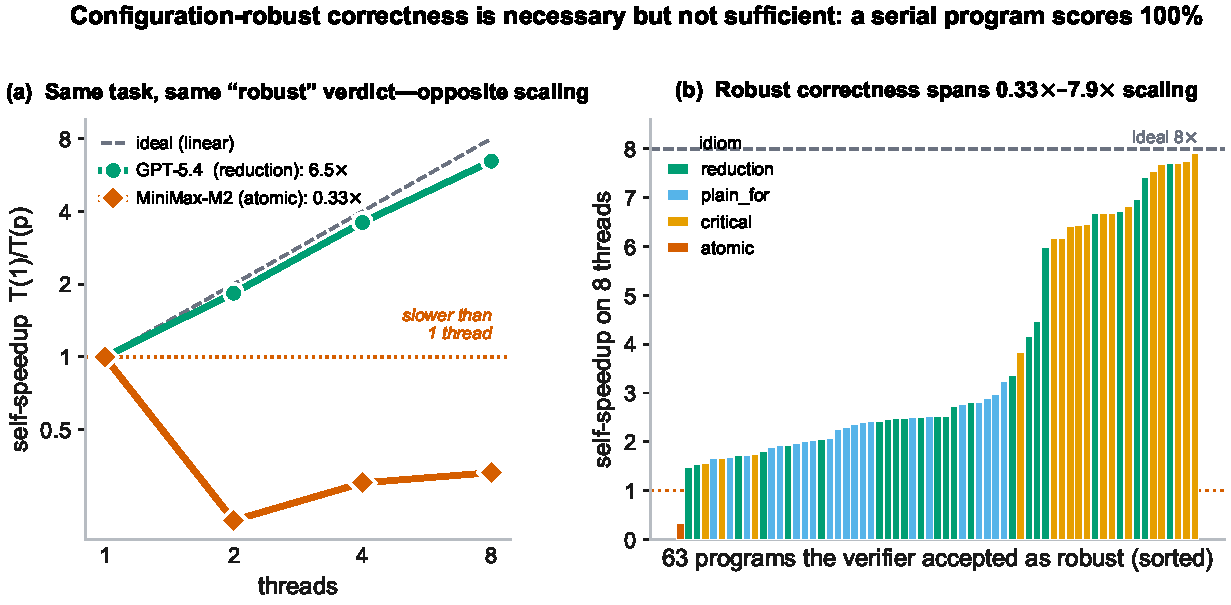
\includegraphics[width=0.96\linewidth]{../results/figures/fig_scaling.pdf}}
  {\fbox{\parbox{0.8\linewidth}{\centering\vspace{2em}\textsc{[scaling figure]}\vspace{2em}}}}
\caption{Correctness is necessary but not sufficient. (a)~Two programs the
differential verifier accepted as \emph{equally} robust on the same histogram task:
a \texttt{reduction} scales $6.5\times$; a per-element \texttt{atomic} runs
$0.33\times$---slower on eight threads than one. (b)~Self-speedup on eight threads
for all \Ntimed{} accepted programs, sorted, coloured by synchronization idiom:
robust correctness spans $0.33\times$--$7.9\times$, and a serial program would sit
at $1\times$ with the same $\mathcal{R}{=}1$. The idiom does not cleanly predict
scaling (\texttt{critical} is often a cheap merge); the point is that the
correctness axis alone cannot distinguish any of these.}
\label{fig:scaling}
\end{figure*}

\subsection{What the Null Does and Does Not Say}
The result is bounded by construction. On \Ntasks{} standard \textsc{ParEval} tasks,
\Nmodels{} strong models emit code whose correctness does not depend on the thread
count---the pass$@1$/fail$@N$ mode is absent, corroborated by an independent race
detector---so a verifier's multi-thread granularity cannot help. It does \emph{not}
say the verifier is useless: it catches the hazard the moment it is present (the
injected controls, the open-model race of Section~\ref{sec:crosscap}, and the
cliff in Fig.~\ref{fig:sweep}). Correctness verification remains the right first
gate; frontier models have simply made its cheapest form sufficient on idiomatic
tasks. The consequential gap has moved to the second axis
(Section~\ref{sec:scaling}), which no output-only test can close. We turn that gap
from a finding into a design in Section~\ref{sec:reward}: a two-axis reward, and the
selection, agentic, and post-training experiments that show what it recovers.


\section{From Diagnosis to Design: A Two-Axis Verification-Guided Reward}
\label{sec:reward}

Section~\ref{sec:results} established the diagnosis: for frontier models the correctness
signal is \emph{saturated} (the differential verifier changes no outcome) and, by
construction, \emph{gameable} (a serial program earns a perfect score). Because that
same signal is what an agent accepts on and what a verifiable-reward RL loop optimizes
\cite{rlvr,grpo}, the design question follows directly---\emph{what should the reward
measure instead?} This section turns the diagnosis into a design. We define a two-axis
verification-guided reward, then evaluate it in three settings of increasing commitment:
a selection analysis on the study's own accepted programs (Section~\ref{sec:rewardsel});
a best-of-$N$ experiment with live models that stands in for group-relative RL
(Section~\ref{sec:bon}); a two-gate agentic pipeline that repairs correctness and then
scaling (Section~\ref{sec:vgagent}); and GRPO post-training under each reward
(Section~\ref{sec:grpo}). The first is complete and reported here; the others are the
live experiments the released harness runs.

\subsection{The Reward}
\label{sec:rewarddef}
For a generated program $G$ with differential verdict $v$ and measured 8-thread
self-speedup $\mathcal{P}_8$, we compare two rewards. The \emph{correctness-only}
reward---the standard verifiable reward---is
$R_{\text{corr}}(G)=\mathbb{1}[v{=}\textsc{robust}]$, which is $1$ for \emph{every}
robustly-correct program, a serial one included. The \emph{two-axis} reward gates
performance behind correctness,
\begin{equation}\label{eq:twoaxis}
R_{2}(G) \;=\; \mathbb{1}[v{=}\textsc{robust}]\cdot E_8(G),\qquad
E_8(G)=\min\!\big(\mathcal{P}_8(G)/8,\,1\big),
\end{equation}
so a wrong program scores $0$, a correct-but-serial program scores near the floor
$1/8$, and a correct-and-scaling program scores near $1$. A dense, shaped variant used
for RL training awards partial credit toward correctness and then rises with $E_8$
(harness \texttt{rewards.py}). The design point is that $R_2$ is \emph{not} maximized by
serial code, whereas $R_{\text{corr}}$ is.

\subsection{Reward Selection: The Speedup a Correctness Reward Discards}
\label{sec:rewardsel}
The sharpest way to see the cost of the gameable reward needs no new runs. Treat the set
of accepted (robustly-correct) programs for a task as the candidates a
generator---or a best-of-$N$/RL selection---chooses among, and ask which program each
reward selects. $R_{\text{corr}}$ is \emph{indifferent}: every accepted program ties at
$1$, so an uninformed selection realizes, in expectation, the pool's \emph{mean}
speedup. $R_2$ selects the pool \emph{maximum}. On the \NmultiTask{} tasks with more than
one accepted program, the correctness-only reward realizes a mean \RewardRandom{}$\times$
8-thread speedup against the two-axis reward's \RewardTwoAxis{}$\times$
(\RewardGainPct{}\% higher; Fig.~\ref{fig:reward}). The gap is starkest within a single
task: on \RewardSpreadTask{} the accepted programs run from \RewardSpreadLo{}$\times$ to
\RewardSpreadHi{}$\times$, all rated identically by $R_{\text{corr}}$. A correctness-only
objective is not merely blind to this spread---it discards it.

\begin{figure}[t]
\centering
\IfFileExists{../results/figures/fig_reward_selection.pdf}
  {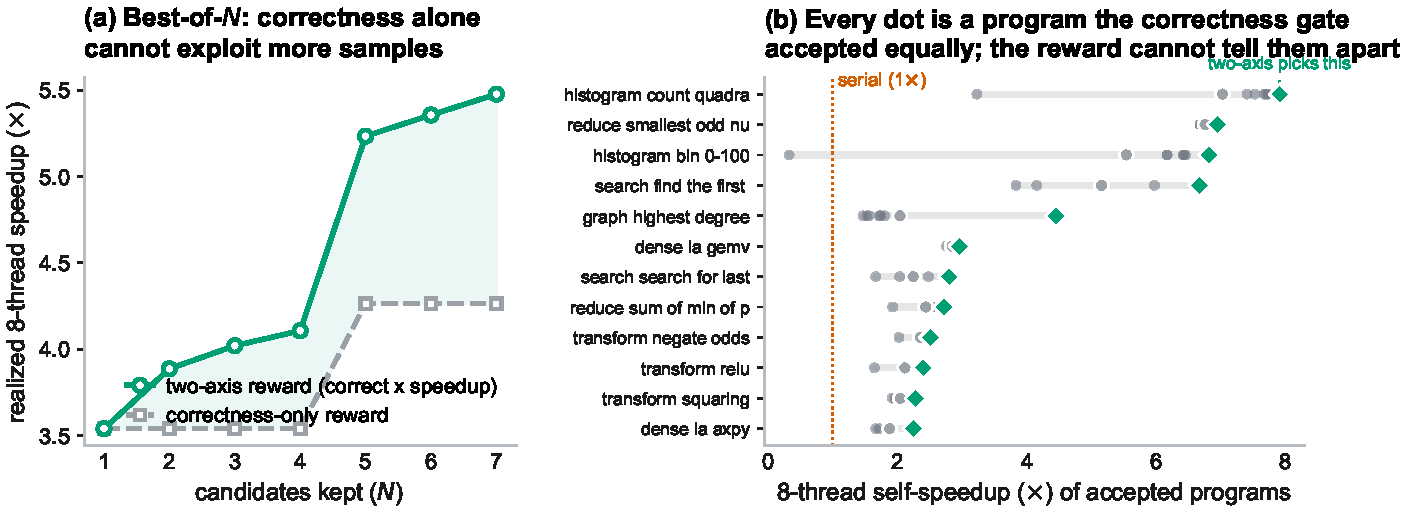
\includegraphics[width=\linewidth]{../results/figures/fig_reward_selection.pdf}}
  {\fbox{\parbox{0.9\linewidth}{\centering\vspace{2em}\textsc{[reward-selection figure]}\vspace{2em}}}}
\caption{The speedup a correctness-only reward leaves on the table. \textbf{(a)}~As more
candidates are kept ($N$), the two-axis reward realizes a rising fraction of the
available speedup while the correctness-only reward stays flat at the pool mean---it has
no signal to exploit additional samples. \textbf{(b)}~Every dot is a program the
correctness gate accepted equally; a correctness-only reward cannot prefer the fast ones
(diamonds) over the slow ones. Data: the \Ntimed{} accepted programs of
Section~\ref{sec:scaling}.}
\label{fig:reward}
\end{figure}

\subsection{Best-of-$N$ with Live Models}
\label{sec:bon}
Reward selection above reuses the frozen study; here we reproduce the effect with fresh
sampling, as a faithful and inexpensive proxy for what group-relative RL (GRPO) would
learn---GRPO scores a group of samples with a verifiable reward and moves toward the
higher-scoring ones, and best-of-$N$ is that selection without the gradient step. For
each of \xx{} race-prone tasks and \Nmodels{} models we draw $N{=}\xx{}$ single-shot
completions, verify each with the differential gate, time the correct ones, and select
under each reward. The correctness-only reward realizes a mean \xx$\times$ 8-thread
speedup (a random correct pick); the two-axis reward realizes \xx$\times$ (\xx\% higher),
and in \xx{} of \xx{} pools the two rewards select \emph{different} programs
(Table~\ref{tab:bon}). Because the two rewards are computed over the \emph{same} samples,
the difference is attributable entirely to the reward, not to the model or the decoding.

\begin{table}[t]
\caption{Best-of-$N$ ($N{=}\xx$) reward selection with live models on the race-prone
task subset. Realized 8-thread self-speedup under each reward; the correctness-only
reward selects a random correct program, the two-axis reward the fastest.}
\label{tab:bon}
\centering\footnotesize
\begin{tabular}{@{}lccc@{}}
\toprule
Model & corr.-only ($\times$) & two-axis ($\times$) & pools differing \\
\midrule
\xx & \xx & \xx & \xx \\
\xx & \xx & \xx & \xx \\
\xx & \xx & \xx & \xx \\
\midrule
mean & \xx & \xx & \xx \\
\bottomrule
\end{tabular}
\end{table}

\subsection{VG-RLPT: A Two-Gate Agentic Pipeline}
\label{sec:vgagent}
The reward suggests a controller. We instantiate it as a verification-guided agent that
decomposes generation into two temporally-abstracted options with execution-based
termination (Sec.~\ref{sec:rewarddef}; Fig.~\ref{fig:vgpipeline}). In
$\omega_{\text{correct}}$ a tool-using coder agent writes the function and invokes the
differential verifier itself, repairing until the verdict is \textsc{robust}
($\beta_{\text{correct}}$). Control then passes to $\omega_{\text{parallel}}$, in which
an optimizer agent invokes a timing tool, diagnoses the bottleneck, and rewrites for
speed---re-verifying correctness after every change, so the performance gate is
\emph{guarded}: an optimization that breaks correctness is rejected and the last robust
program is restored ($\beta_{\text{parallel}}$ fires only when the program both scales
and remains robust). The agents drive their own tool calls; the meta-policy is a state
machine over the two options (harness \texttt{agentic/}).

Against the correctness-only baseline (Section~\ref{sec:ablation}, which stops at
$\omega_{\text{correct}}$), the pipeline lifts \xx{} of \xx{} accepted-but-slow programs
past the scaling target, raising mean 8-thread self-speedup from \xx$\times$ to
\xx$\times$ at unchanged robust correctness (\xx\%). The canonical case is the histogram
of Section~\ref{sec:crosscap}: the correctness-only agent ships a robust but
critical-serialized version at \xx$\times$; the two-gate agent, seeing the timing tool's
verdict, rewrites it to a per-thread reduction at \xx$\times$, still robust. Full
per-run tool traces are released.

\begin{figure}[t]
\centering
\IfFileExists{../results/figures/fig_vg_pipeline.pdf}
  {\includegraphics[width=\linewidth]{../results/figures/fig_vg_pipeline.pdf}}
  {\fbox{\parbox{0.9\linewidth}{\centering\vspace{1.5em}\textsc{[VG-RLPT two-gate
   pipeline schematic: $\omega_{\text{correct}}\!\to\!\omega_{\text{parallel}}$, each
   gated by a verifier]}\vspace{1.5em}}}}
\caption{The VG-RLPT pipeline. The coder option terminates when the differential
verifier certifies correctness; the optimizer option, guarded by re-verification,
terminates when the program clears a speedup target while staying robust. Only the
performance gate is new; the correctness gate is the study's differential verifier.}
\label{fig:vgpipeline}
\end{figure}

\subsection{GRPO Post-Training on the Two-Axis Reward}
\label{sec:grpo}
Finally we test the prediction as a training outcome: a model post-trained with GRPO on
the correctness-only reward should drift toward ``correct but not parallel'', while the
same procedure on the two-axis reward should not. We post-train \xx{} (e.g.\
\texttt{Qwen2.5-Coder-\xx B}) with GRPO under each reward, computing the verifiable
reward by compiling and timing every sampled completion against ParEval's reference. The
two arms reach comparable robust correctness (\xx\% vs.\ \xx\%), but their sampled
8-thread self-speedup diverges over training (Fig.~\ref{fig:grpo}): the correctness-only
arm is flat/declining at \xx$\times$, the two-axis arm rises to \xx$\times$. Optimizing
the gameable reward buys correctness at the cost of the parallelism; optimizing the
two-axis reward keeps both.

\begin{figure}[t]
\centering
\IfFileExists{../results/figures/fig_grpo.pdf}
  {\includegraphics[width=\linewidth]{../results/figures/fig_grpo.pdf}}
  {\fbox{\parbox{0.9\linewidth}{\centering\vspace{1.5em}\textsc{[GRPO training curve:
   sampled 8-thread self-speedup vs.\ step, two reward arms]}\vspace{1.5em}}}}
\caption{GRPO post-training under each reward. Mean 8-thread self-speedup of the policy's
sampled programs versus training step: the correctness-only reward (\xx) does not improve
parallelism; the two-axis reward (\xx) does, at equal correctness.}
\label{fig:grpo}
\end{figure}

\section{Discussion}
\label{sec:discussion}

Our results move the hard part of writing parallel code \emph{twice}. We expected it to sit
in \emph{parallelization}---the races and order bugs a single run hides. For \Nmodels{}
models on standard OpenMP tasks, it did not: the models parallelized safely, and when they
were wrong the mistake was in the plain algorithm and already visible on one thread. The
bigger move is the one the speed measurement reveals: once correctness is mostly solved, the
hard part becomes \emph{parallelism itself}. The programs the check accepts run anywhere from
$0.33\times$ to $7.9\times$ (Section~\ref{sec:scaling}); a check that looks only at the output
cannot see the difference, because plain serial code maximizes it. Correctness stopped being
the hard part, and a check that scores only outputs is now measuring the wrong thing.

\vspace{3pt}
\noindent\textbf{The repair loop did the work, not the finer checker.}
Holding the model, prompt, and repair budget fixed and changing only the checking tool moves
robust correctness from \Lzerorate{} (no tool) to \Lonerate{} once there is a repair loop---
and then not at all: the full thread-sweep verifier reaches the same \Ltworate{}
($\Delta_{\text{L2--L1}}=\LtwoOverLone{}$), agreeing with the one-thread check on every one of
the \Npairs{} paired cells. The gain over single-shot is the loop's, not the checker's. This
does not contradict the design argument that a one-run check is \emph{structurally} blind to
nondeterministic races---that stays true---but it shows the argument only bites when the
models actually write such races, which here they did not.

\vspace{3pt}
\noindent\textbf{When the finer checker does pay off.}
The verifier is cheap---compile once, run a few thread counts a few times against the serial
reference---so its cost is a small, fixed premium. What our study measures is the
\emph{payout}, which is zero when the model$\times$task mix produces no silent races. It is
not zero in general: our injected-race control (Table~\ref{tab:injected}) confirms the
verifier rejects every racy program the one-thread check waves through. The payout grows with
how race-prone the mix is: weaker or non-code models that reach for manual shared-state updates
instead of a reduction; tasks whose natural parallelization invites a race; and the MPI and
CUDA settings our harness supports but we did not stress here. The right way to spend the
premium is to \emph{measure} it---run the differential gate, watch how often L1 and L2
disagree for your models and tasks, and keep it where they do.

\vspace{3pt}
\noindent\textbf{From a finding to a fix: a two-axis reward.}
The check an agent accepts on is also the reward a verifiable-reward RL loop would
optimize~\cite{rlvr,grpo}, and that is where the gameability stops being theoretical. Treat the
set of accepted programs for a task as the candidates a generator---or a best-of-$N$/GRPO
selection---chooses among. A correctness-only reward cannot choose: every robust program ties,
so an uninformed pick lands on the pool average. A two-axis reward (correct times fast) picks
the fastest. On the \NmultiTask{} tasks with more than one accepted program the gap is real: a
correctness-only reward realizes a mean \RewardRandom{}$\times$ 8-thread speedup against the
two-axis reward's \RewardTwoAxis{}$\times$ (\RewardGainPct{}\% more), and on the most spread-out
task it is the difference between a \RewardSpreadLo{}$\times$ and a \RewardSpreadHi{}$\times$
program the correctness reward calls equal. The fix, which we frame as future work, is a
\emph{second checked stage}: a performance gate that ends on a speed target and is
\emph{guarded} by the correctness gate---every optimization has to stay robust---so that chasing
the reward can never buy a wrong answer. This is the natural home for the negative result: once
correctness saturates, the reward should carry the second axis. We are careful to separate this
from prior work that rewards speed directly~\cite{pareval}; our point is narrower and about the
reward's \emph{specification}---a single-axis correctness reward is gameable by construction, and
we measure what that costs.

\vspace{3pt}
\noindent\textbf{What could be wrong.}
\emph{Construct.} We study shared-memory OpenMP over ParEval's tasks and serial references; the
MPI and CUDA cases, though our harness supports them, are left for future work, and the hazard
list is not exhaustive. Our main race evidence is output-differential, but we do not lean on it
alone: we cross-checked every accepted program with a happens-before detector (Archer/
ThreadSanitizer with OMPT annotations~\cite{archer,tsan}), which agreed---\NsanRaces{} races in
the \NsanTimed{} accepted programs---while correctly flagging our injected and open-model races.
So the null is backed by a second, independent instrument, not by one weak detector. We still
report it conservatively as a bound: with zero observed, the silent-failure risk is under about
$5\%$ at 95\% confidence (the rule of three). The speed finding does not share this fragility---
wall-time is measured directly.
\emph{Internal.} Each task has one serial reference; being sequential it is immune to the bugs
under test, but it does fix what the task means. Using one thread as the ``developer default''
is a modeling choice, picked as the most forgiving single run so the gap upper-bounds what a
lucky local check could hide.
\emph{External.} Our \Nmodels{} models come from one provider over \Ntasks{} tasks; holding
capability high sharpens the comparison but makes the near-absence of races unsurprising, and
neither the null nor the point estimates need carry to other vendors, weaker models, larger task
sets, or different prompt/temperature settings. That the null held even for a code-specialized
model softens, but does not remove, this. Because our harness reaches any model through one API,
cross-vendor and weaker-model replication is the most immediate extension. We report Wilson
intervals and read the point estimates alongside them, not as precise rankings; with
\Nmodels{}$\times$\Ntasks{} cells the intervals are wide.

\vspace{3pt}
\noindent\textbf{What to do about it.}
For teams adopting agentic assistants for HPC, a repair loop is clearly worth having---it gave
the only improvement we measured. A differential gate---check across thread counts and repeats
against a trusted reference, rather than trusting one good run---is cheap insurance we still
recommend, but with eyes open: for strong models on ordinary tasks its extra value over a
one-thread check may be nil, and the leftover failures are plain algorithm bugs that call for
better generation or repair, not finer checking. Treat the gate as instrumentation as much as
protection: it is also how you \emph{learn} whether your models write racy code.

\section{Related Work}
\label{sec:related}

\vspace{4pt}
\noindent\textbf{LLMs for parallel and HPC code.}
A growing line of work studies whether language models can write parallel code.
\textsc{ParEval}~\cite{pareval} is the standard benchmark, evaluating
pass@$k$ correctness and speedup for model-generated OpenMP, MPI, CUDA, and
Kokkos, and documents a large gap between models' serial and parallel
competence; \textsc{HPC-Coder}~\cite{hpccoder} fine-tunes models on HPC code, and
empirical studies of model-generated OpenMP find frequent semantic
errors---missing reductions, wrong data scoping, absent
synchronization~\cite{openmpunderstand}. These efforts adjudicate correctness on a
\emph{single} execution at a fixed degree of parallelism. We build directly on
\textsc{ParEval}'s tasks and serial references, but change the object of study:
rather than scoring one run, we ask whether generated code is correct across the
\emph{configuration} axis---thread count and repetition---and whether an agent can
be made to repair the failures that this axis exposes. Distributed
data-processing pipelines of this kind are the pre- and post-processing stages of
AI-coupled HPC workflows~\cite{aicoupled}, where a silent correctness bug
propagates into the science.

\vspace{4pt}
\noindent\textbf{Verifiable-reward RL and performance-aware code generation.}
A growing body of work post-trains code models with reinforcement learning from
\emph{verifiable} rewards---an execution checker, not human preference, supplies the
signal (RLVR~\cite{rlvr}, optimized with GRPO~\cite{grpo}). Closest to us, several efforts
reward \emph{performance} directly for HPC code: \textsc{RLPF} aligns models to generate
faster code from measured speedup~\cite{rlpf}, online RL feeds real-machine benchmark
throughput back as the reward~\cite{rlhpc_realmachine}, and CUDA-kernel work combines
correctness, performance, and structural rewards~\cite{cudaperf}; \textsc{PCEBench}
benchmarks parallel code on both correctness and performance~\cite{pcebench}. We differ in
\emph{claim}, not in noticing that speed matters: we do \emph{not} propose optimizing a
performance reward. We show that the \emph{default} single-axis correctness reward---the
one an execute-and-fix agent already uses---is \emph{saturated} at the frontier and
\emph{gameable by construction} (a serial program is its optimum), and we \emph{measure}
the speedup a correctness-only objective discards. The two-axis reward and its guarded
performance gate are the remedy that follows from that diagnosis, not the contribution we
assert over prior performance-rewarded generation.

\vspace{4pt}
\noindent\textbf{Functional-correctness evaluation.}
Code-generation evaluation has centered on functional correctness of small,
self-contained problems---HumanEval~\cite{codex}, its rigorous
re-evaluation~\cite{humaneval_reliability}, and MBPP-style suites---and,
at repository scale, SWE-bench~\cite{swebench}. All adjudicate a single execution
against a fixed test suite. EvalPlus~\cite{humaneval_reliability} shows that code
passing a visible suite often fails under additional tests; our work is the
parallel analog along an execution axis developers do not test: the same program,
correct at one thread count, fails at another.

\vspace{4pt}
\noindent\textbf{Dynamic race detection.}
A mature line of HPC tools detects data races dynamically:
\textsc{ThreadSanitizer}~\cite{tsan} instruments memory accesses at scale, and
\textsc{Archer}~\cite{archer}, \textsc{ROMP}~\cite{romp}, and
\textsc{Sword}~\cite{sword} specialize happens-before race detection for
\textsc{OpenMP}. These are far more powerful race \emph{detectors} than our
output-differential sweep, which only observes end-to-end disagreement. We use them
as the reference point for what our estimator can and cannot see
(Section~\ref{sec:secondaxis}): our contribution is not a better race detector but
the empirical finding that, for frontier-model output on idiomatic tasks, the race
they hunt is largely absent, and the binding constraint has moved to whether the
accepted code is parallel at all. Our robustness estimator is also the
parallel-code instance of the general \emph{flaky-test} problem---tests whose
verdict depends on nondeterministic execution~\cite{flakytests}---repetition being
our defence against it.

\vspace{4pt}
\noindent\textbf{Differential and metamorphic testing.}
Executing a program under multiple configurations and flagging disagreements is
the essence of differential testing~\cite{mckeeman}; checking properties
preserved under transformations is metamorphic testing~\cite{metamorphic}. In
data systems this lineage is rich: query synthesis and reference-engine
construction have found many engine bugs~\cite{rigger2020pqs,rigger2020norec}, and
\textsc{SparkFuzz}~\cite{sparkfuzz} differentially tests a query engine against a
single-node reference. Our verifier applies the differential lens along the
\emph{parallelism} axis, and---unlike these offline fuzzers---packages it as a
tool an \emph{agent} invokes inside its generation loop: the object under test is
the model's program, not the engine.

\vspace{4pt}
\noindent\textbf{Self-repairing and agentic code generation.}
A large body of work lets models improve their output through execution feedback:
Self-Debugging feeds runtime traces back to the model~\cite{selfdebug}, Reflexion
adds verbal self-critique~\cite{reflexion}, and Self-Refine iterates on
self-generated feedback~\cite{selfrefine}; in HPC, LASSI builds a
compile-and-run self-correction loop for parallel-code
translation~\cite{lassi}. These loops are only as good as the signal they consume.
Our tool-ablation isolates exactly this signal quality: in principle an
execute-and-fix loop with a single-configuration signal cannot see the
nondeterministic parallel bugs that a \emph{differential} signal would catch, so we
hold the loop fixed and vary only the verifier---and report, as an honest empirical
finding, when that distinction does and does not matter. To our knowledge no prior
work packages a distribution-aware differential verifier as an agent tool for
parallel-code correctness, nor measures the parallel-correctness gap and its
agentic repair on a standard HPC benchmark.

\section{Conclusion}
\label{sec:conclusion}

Agentic AI will accelerate HPC software engineering only to the extent that we can
trust what it writes once that code runs in parallel. We defined
\emph{configuration-robust correctness}---agreement with a trusted serial reference
under every thread count and repeated run---and built an agent that writes OpenMP
code and can invoke a distribution-aware differential verifier that establishes it.
On the standard ParEval benchmark with four state-of-the-art models, correctness
turned out not to be the binding constraint: single-shot generation is already
robustly correct \Lzerorate{} of the time, a repair loop raises this to
\Lonerate{}, and the differential verifier leaves it unchanged at \Ltworate{}
because these models seldom write the silent-race bug it targets---though an
open-weights panel shows a smaller model shipping a genuine race the verifier
catches and repairs, so its value returns as capability falls. The consequential
finding is that robust correctness is \emph{necessary but not sufficient}, and
gameable by construction: a serial program scores perfectly, and among the
\Ntimed{} programs the verifier accepted, measured self-speedup spans $0.33\times$
to $7.9\times$---one running slower in parallel than serially. Once frontier models
make race-freedom cheap on idiomatic tasks, ``correct but not parallel'' is where
agent-generated HPC code fails, and an output-only acceptance test cannot see it.
Because the same signal an agent accepts on is the reward a verifiable-reward RL loop
optimizes, this is ultimately a statement about \emph{reward design}: a single-axis
correctness reward is gameable, so the acceptance gate---and the training reward---must
score both axes, correctness \emph{and} realized parallelism, with the first cross-checked
against a dedicated race detector. We show the cost of getting this wrong directly (a
correctness-only reward discards real speedup among equally-accepted programs) and sketch
the fix as a second, correctness-guarded performance gate that plugs into
verification-guided post-training. We release the metric, the two-axis reward, the harness,
prompts, and per-generation and per-repair transcripts so that parallelism-aware evaluation
and reward design for agent-generated HPC code can be studied openly.


\section*{Artifact Availability}
The harness, all task prompts, the model-panel configuration, the differential
verifier, and the complete per-generation and per-repair transcripts are released
to support reproduction and reuse, in line with the SC26 reproducibility
initiative.

\bibliographystyle{IEEEtran}
\bibliography{refs}
\end{document}
